\documentclass{article}%
\usepackage[T1]{fontenc}%
\usepackage[utf8]{inputenc}%
\usepackage{lmodern}%
\usepackage{textcomp}%
\usepackage{lastpage}%
\usepackage{authblk}%
\usepackage{graphicx}%
%
\title{Decursin Isolated from Angelica gigas Nakai Rescues PC12 Cells from Amyloid \_\_{-}Protein{-}Induced Neurotoxicity through Nrf2{-}Mediated Upregulation of Heme Oxygenase{-}1: Potential Roles of MAPK}%
\author{Manuel Schmidt}%
\affil{Zhang Zhongjing College of Chinese Medicine, Nanyang Institute of Technology, China}%
\date{01{-}01{-}2013}%
%
\begin{document}%
\normalsize%
\maketitle%
\section{Abstract}%
\label{sec:Abstract}%
The ability of molecular investigators to accurately diagnose cancer in the same head{-}to{-}head world as in the blood is in jeopardy because current diagnostic tests are biased toward blood glucose due to the error rate of sample sampling.\newline%
In new research led by Dr. Brian Whitney, of Massachusetts General Hospital, researchers demonstrated a new molecular mechanism of SSR128129E that inhibits FGF signaling. Dr. Whitney and colleagues identified a new molecule on the surface of tumors called SSR128129E

%
\subsection{Image Analysis}%
\label{subsec:ImageAnalysis}%


\begin{figure}[h!]%
\centering%
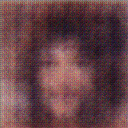
\includegraphics[width=150px]{500_fake_images/samples_5_284.png}%
\caption{A Black And White Cat Is Sitting On The Ground}%
\end{figure}

%
\end{document}